% Working paper: LaTeX version of ../pls_action_units.md
% Build:  cd paper/latex && pdflatex main && bibtex main && pdflatex main && pdflatex main
\documentclass[11pt,a4paper]{article}

\usepackage[T1]{fontenc}
\usepackage[utf8]{inputenc}
\usepackage{lmodern}
\usepackage{microtype}
\usepackage[margin=2.5cm]{geometry}
\usepackage{amsmath,amssymb,bm}
\usepackage{graphicx}
\usepackage{booktabs}
\usepackage{tabularx}
\usepackage{array}
\usepackage[font=small,labelfont=bf]{caption}
\usepackage[round,authoryear]{natbib}
\usepackage{xcolor}
\usepackage[colorlinks=true,linkcolor=blue!50!black,citecolor=blue!50!black,urlcolor=blue!50!black]{hyperref}

\graphicspath{{../figures/}}
\setlength{\parskip}{0.4em}
\setlength{\parindent}{0pt}
\newcommand{\Cov}{\operatorname{Cov}}
\newcommand{\SNR}{\mathrm{SNR}}
\newcommand{\code}[1]{\texttt{#1}}
\let\olditemize\itemize
\renewcommand{\itemize}{\olditemize\setlength{\itemsep}{0.15em}\setlength{\parskip}{0pt}}

\title{Why a low-dimensional linear model wins in real time:\\[0.2em]
\large landmark noise, expression dimensionality and action units in geometric affect regression}
\author{Vassilios Vonikakis\\[0.3em]
\small Analyses and draft prepared with Claude (Anthropic)}
\date{Working paper, November 2026}

\begin{document}
\maketitle

\begin{abstract}
\noindent A linear Partial Least Squares (PLS) regressor with 31 components, applied to pairwise
distances between 51 facial landmarks, estimates arousal, valence and intensity in real time. Two
observations motivated this study: 31 is close to the number of facial action units (AUs)
defined by the Facial Action Coding System, and in a live webcam demo the 31-component model
behaves better than models that are more accurate in cross-validation, including ridge and RBF
kernel ridge regression. We measure the landmark detector's noise directly, using mirrored image
copies as independent re-detections of the same faces, and separate expression signal from noise
in 83,191 images of 337 people. One dlib detection has about 1\,px of noise per coordinate,
concentrated in a few whole-shape directions. Within-person expression deformations exceed four
times this noise in about 20 directions and twice the noise in about 30. The first $\sim$20 PLS
components match action-unit templates; after that, AU structure, replicability and
signal-to-noise fade together. The accuracy-optimal complexity depends on the noise: on still
photographs cross-validation prefers the most complex models, but at 3.2 times the noise of one
detection, which our simulation gives for the original detector in a dim webcam scene, the optimum
drops to 32 PLS components, or a ridge model with 104 effective degrees of freedom that behaves
like PLS(31). Extra complexity also costs jitter and pose stability, and a kernel model responds
about 12 times less consistently to the same synthetic action unit across faces. A ridge model of
matched complexity matches or beats PLS(31) on every measure. The number of action units thus
turns out to be a good proxy for the number of facial movements a landmark detector resolves, and
models for interactive affect estimation should be selected at the noise level of deployment and
tested for the behaviour users see.
\end{abstract}

\noindent\textbf{Reproduce:} every number and figure comes from
\nolinkurl{experiments/14_pls_dimensionality.py} (about 10 minutes on a laptop CPU).\\
\textbf{Code and data:} \url{https://github.com/bbonik/facial-expression-analysis}.

% ==========================================================================================
\section{Introduction}

Geometric facial-expression models map facial landmarks to affect. In the system studied here,
dlib's 68-point landmarks \citep{kazemi2014one} are normalised for position, scale and in-plane
rotation, frontalized by a linear map \citep{vonikakis2020frontalization}, and turned into 1,275
distances between the 51 non-jaw landmarks. The distances are divided by a scale measured on
expression-stable points. A regressor then predicts arousal, valence and intensity, the
dimensions of Russell's circumplex model of affect \citep{russell1980circumplex,
vonikakis2021efficient}. The regressor is trained on MorphSet \citep{vonikakis2021morphset}, whose
dimensional labels are generated by morphing each person's neutral face towards their posed
expressions.

The original 2021 system used PLS \citep{wold2001pls} with 31 components. This number was not
chosen by cross-validation. It was the author's choice: roughly the number of facial action
units, and the model that behaved best in a live demo. A modern evaluation of the same system
found that nested cross-validation prefers about 50 components; that ridge and RBF kernel ridge
regression are more accurate in person-grouped cross-validation and when generalising to a
held-out database; and that PLS(31) nevertheless behaves better on new faces. Its neutral faces
land nearer the origin, a synthetic smile moves along the valence axis, and outputs vary less
across head pose.

This paper asks why. Specifically:
\begin{itemize}
  \item[\textbf{Q1}] How large is the landmark noise, and how many independent directions of
  facial expression rise above it?
  \item[\textbf{Q2}] Do PLS components correspond to action units, and up to which component?
  \item[\textbf{Q3}] Why does offline accuracy select a more complex model than live use does,
  and what determines the right complexity?
\end{itemize}
The main tool is a careful separation of \emph{signal} (real changes of facial geometry) from
\emph{noise} (the detector's error), which Section~\ref{sec:signal-noise} shows is possible even
though the detector's output is all we have.

% ==========================================================================================
\section{Data and methods}

\subsection{Data}

\textbf{MorphSet} \citep{vonikakis2021morphset}: 83,191 images of 337 people from RaFD, KDEF,
WSEFEP and FACES. Each person's neutral face is morphed in 10 steps towards 7 basic expressions
and 4 blends. All images are scaled so that the eye centres are 150\,px apart. The dataset ships
dlib landmarks of every image, and of a horizontally mirrored copy of every image
(Section~\ref{sec:signal-noise}). MorphSet's subject ids identify photo series, not people, so all
splits use corrected person ids. Except for the noise measurement, we use the original images
only.

\textbf{Real expressions:} the multi-pose landmark dataset used to train the frontalizer. It covers
Multi-PIE, KDEF and, most likely, CAS-PEAL, with 42,834 shapes of 1,202 people. For dimensionality
we use frontal views (2,323 expressions with a neutral face of the same person). For behaviour
tests we use Multi-PIE and CAS-PEAL people only, because KDEF people also appear in MorphSet:
2,294 neutral frontal faces and 23,795 faces at yaw $\le 45^\circ$. The origin of these landmarks
(detector or manual annotation) is not documented, so their noise is unknown.

\subsection{Signal, noise, and how to separate them}\label{sec:signal-noise}

\paragraph{The problem.} We never observe the true facial geometry. Every shape in the data is the
output of dlib's detector, which adds an error to the true positions of the landmarks:
\begin{equation}
  x = s + e,
\end{equation}
where $x$ is the detected shape (102 numbers: 51 landmarks $\times$ 2 coordinates), $s$ is the true
shape and $e$ is the detection error, with covariance $\Sigma_e$. The variance in any direction of
shape space is the sum of real variation and noise, so no analysis of $x$ alone can tell them
apart. We need an independent measurement of $\Sigma_e$.

\paragraph{Measuring the noise: mirror twins.} MorphSet contains a horizontally mirrored copy of
every image, and dlib detected landmarks on each copy independently. A mirrored face has the same
geometry, flipped. Dlib's HOG face detector and its cascade of regression trees, however, are not
mirror-symmetric. On the mirrored image the detector returns a different box, and the trees take
different branches, so the two detections make different errors on the same face. We undo the
mirror on the second detection, $\tilde x_2$, by negating its x coordinates and swapping the left
and right landmark labels. The difference between the twins is then
\begin{equation}
  d = x_1 - \tilde x_2 = (s + e_1) - (s + e_2) = e_1 - e_2 .
\end{equation}
The true shape cancels, and what remains is pure detection error. If the two errors are
independent with the same covariance, $\Cov(d) = 2\Sigma_e$. We remove the mean of $d$ over all
83,191 pairs, because it is a systematic left/right asymmetry of dlib (0.33\,px rms), not a random
error, and the translation of each pair, which the mirroring changes. $\Sigma_e$ is estimated in
each coordinate system used below: raw pixels, Procrustes-normalised shapes, frontalized shapes
and the 1,275 distance features.

From the same differences we build a \emph{noise bank}: 83,191 vectors $d/\sqrt{2}$, each a
realistic single-detection error with the correct correlations between landmarks. To add
detector-like noise to a face, we draw a random vector from the bank and scale it to the face's
eye distance. All noise simulations in this paper use this bank, not idealised Gaussian noise.

The twin noise captures the part of the error that changes between detections, which is what
appears as frame-to-frame jitter. It misses errors that both detections share, for example when
the image is blurred or ambiguous in a mirror-symmetric way. It is therefore a lower bound on the
total error, but the right quantity for jitter.

\paragraph{Measuring the signal.} Expressions are measured as within-person \emph{deformations}:
an expression shape minus the same person's neutral shape. Each deformation contains two
detections, so
\begin{align}
  \delta &= x_{\text{expr}} - x_{\text{neutral}}
          = (s_{\text{expr}} - s_{\text{neutral}}) + (e_1 - e_2), \\
  \Cov(\delta) &= \Sigma_s + 2\Sigma_e ,
\end{align}
where $\Sigma_s$, the covariance of the true expression changes, is the signal. Because $\Sigma_e$
is measured independently, the signal follows by subtraction,
$\Sigma_s = \Cov(\delta) - 2\Sigma_e$. For neutral faces of different people (identity), only one
detection is involved, and $\Sigma_s = \Cov(x) - \Sigma_e$.

\paragraph{Signal-to-noise ratio.} Along a direction $v$ of shape or feature space we define
\begin{equation}\label{eq:snr}
  \SNR(v) = \frac{v^\top \Sigma_s\, v}{v^\top \Sigma_e\, v}
          = \frac{v^\top \Cov(\delta)\, v}{v^\top \Sigma_e\, v} - 2 ,
\end{equation}
the variance of real expression movement along $v$ divided by the noise variance of one detection
along $v$. This is the relevant ratio for live use. After calibration on many neutral frames, each
new frame carries the noise of one detection. $\SNR = 1$ means that the expression signal along
that direction is as large as the frame-to-frame noise.

\paragraph{Counting dimensions.} To count directions with SNR above a threshold, we use the
generalised eigenvalues of $\Cov(\delta)$ relative to $\Sigma_e$, the maximum-noise-fraction
transform of remote sensing \citep{green1988mnf}. We whiten the coordinates by the noise, so that
noise has unit variance in every direction, and compute principal components of the whitened data.
Each eigenvalue minus 2 is the SNR of one direction, and the directions are uncorrelated in both
signal and noise. This spectrum does not change under any invertible linear map of the
coordinates. Frontalization, being linear, can therefore neither create nor remove dimensions. A
\emph{naive count} instead compares the ordinary eigenvalues of $\Cov(\delta)$ with a single
average noise level, and so depends on how noise is spread across directions. We report both.

With finite samples, eigenvalues spread even without signal. A direction counts as statistically
detectable when its eigenvalue exceeds the Marchenko--Pastur upper edge for pure noise,
$(1+\sqrt{p/n})^2$, with $p$ coordinates and $n$ samples \citep{marchenko1967distribution}.
Detectable does not mean useful. For live use, the thresholds $\SNR > 1$ and $\SNR > 2$ matter more.

\subsection{Action-unit templates}

Without AU-annotated landmark data, we wrote geometric templates for 16 AUs that move the 51
landmarks: AU1, 2, 4, 5, 6, 7, 9, 10, 12, 15, 17, 20, 23, 25, 26 and 27. Each is a symmetric,
unit-norm displacement field derived from the FACS description \citep{ekman2002facs}. For example,
AU12 moves the lip corners up and outwards, and AU5 raises the upper eyelids. The templates encode
direction, not magnitude.

\subsection{Experiments}\label{sec:experiments}

\paragraph{N. Landmark noise.} Mirror-twin differences of all 83,191 image pairs, in pixels (per
region and overall), in normalised shape coordinates and in feature space. To compare with an
earlier simulation of webcam video (Section~\ref{sec:noise}), we also express the twin difference
in that simulation's ``landmark jitter'' units: the mean landmark displacement between two
detections, in percent of the outer eye-corner distance.

\paragraph{A. Intrinsic dimension.} The noise-whitened SNR spectrum for three sets of 51-landmark
shapes: apex MorphSet expressions minus the same person's neutral face (8,248 deformations); real
frontal expressions minus neutral (2,323); and neutral faces of different people as a reference
for identity (711). We compute it after frontalization and with Procrustes normalisation only,
since MorphSet faces are frontal anyway. The twin noise does not apply to the real-expression
dataset, whose landmarks come from a different source; for it we report only the naive count,
which uses the same yardstick for morphed and real expressions.

\paragraph{B. What PLS components encode.} A PLS model with 60 components is fitted to the
standardised features of all MorphSet images. For each component we compute:
\begin{itemize}
  \item \emph{facial movement:} the minimum-norm landmark displacement that produces the
  component's feature loading, by least squares through the Jacobian of the distances on the mean
  face;
  \item \emph{AU match:} the absolute cosine between the movement and the best AU template, against
  a null from 300 random feature-space directions (95th percentile 0.31);
  \item \emph{AU coverage:} the share of each template's energy in the span of the first $k$
  component movements, compared with $k$ random directions;
  \item \emph{localisation:} one minus the normalised entropy of the movement's energy over facial
  regions, counted as localised above the random-direction 95th percentile;
  \item \emph{replicability:} the best absolute cosine of each component with any component of a
  PLS fit on the other half of the people (two splits), and the subspace stability (mean squared
  cosine of the principal angles between the spans of the first $k$ components);
  \item \emph{identity share:} the score variance across people's neutral faces divided by that
  variance plus the variance of within-person deformations.
\end{itemize}

\paragraph{C. SNR along each PLS component.} For a weight vector $w$ in standardised feature space,
the observed deformation variance is $w^\top\Cov(\delta)w$ and the noise variance $w^\top\Sigma_e w$
is estimated from feature differences of 12,000 twin pairs, halved. The SNR follows from
Eq.~\eqref{eq:snr}.

\paragraph{D. Accuracy versus live behaviour.} Models: PLS with $k = 1$--60 components; ridge with 13
penalties from $10^{-7}$ to $10^{-1}$ per sample, with effective degrees of freedom
$\sum_i \lambda_i/(\lambda_i + \alpha n)$ \citep{hastie2009elements}; and RBF kernel ridge with a
Nystr\"om basis of 2,000 faces, $\gamma = 0.5/1275$ and $\alpha = 1$, chosen earlier by nested
cross-validation. \emph{Accuracy} is the concordance correlation coefficient
\citep[CCC;][]{lin1989concordance} in 5-fold cross-validation grouped by person, averaged over
arousal, valence and intensity; \emph{delta CCC} uses responses relative to the person's own
neutral face, which removes person-specific offsets. \emph{Behaviour} is measured on unseen
Multi-PIE and CAS-PEAL people, with models trained on all of MorphSet:
\begin{itemize}
  \item \emph{identity leakage:} the standard deviation of (A, V) across neutral faces of
  different people;
  \item \emph{AU response heterogeneity:} each AU template, at 6\% of the eye distance, is applied
  to every neutral face; the share of the variance of the resulting (A, V) changes that differs
  between faces (0: identical response for everyone);
  \item \emph{jitter:} the mean $|\Delta A|, |\Delta V|$ when one noise-bank vector is added to each
  neutral face, averaged over three draws;
  \item \emph{pose sensitivity:} the standard deviation of (A, V) across yaw angles for the same
  person and expression.
\end{itemize}

\paragraph{E. Accuracy at webcam noise levels.} Webcam frames are noisier than still photographs:
sensor noise, compression and motion blur, often in poor light. We take 15,000 random MorphSet
images, add noise-bank vectors scaled by $m = 1, 2, 3$ to their raw landmarks (total noise
$\sqrt{1+m^2}$ = 1.4, 2.2 and 3.2 times one detection), and feed them to the models of each
cross-validation fold, which were trained on the original images. For each noise level we record
the CCC of every model and the complexity that maximises it.

% ==========================================================================================
\section{Results}

\subsection{\texorpdfstring{The landmark noise is about 1\,px and concentrated in a few directions}{The landmark noise is about 1 px and concentrated in a few directions}}\label{sec:noise}

\begin{figure}[t]
  \centering
  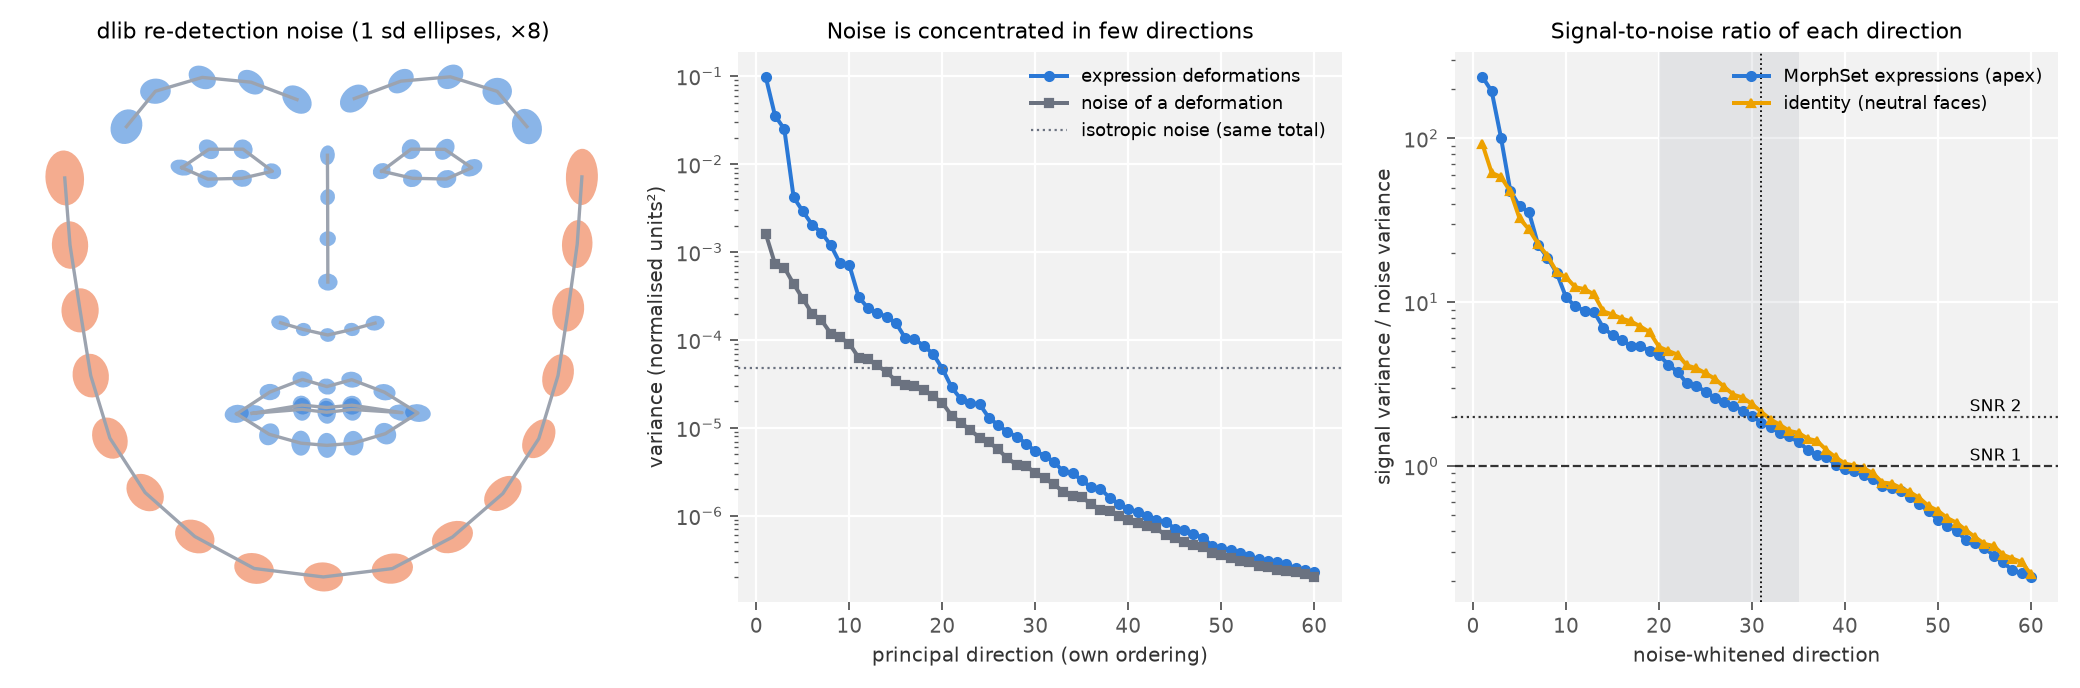
\includegraphics[width=\textwidth]{fig1_spectra.png}
  \caption{Left: dlib's re-detection noise per landmark, measured from mirror twins (1\,sd
  ellipses, magnified 8 times; jaw in orange). Middle: variance of the principal directions of
  expression deformations (MorphSet, apex) and of the noise of a deformation, each sorted by size;
  dotted: isotropic noise of the same total. Right: SNR of each noise-whitened direction for
  MorphSet expressions and identity. Shaded: directions 20--35; dotted vertical line: 31.}
  \label{fig:noise}
\end{figure}

\begin{table}[h]
  \centering\small
  \caption{Noise standard deviation of one dlib detection, per coordinate, at a 150\,px eye
  distance.}\label{tab:noise}
  \begin{tabular}{lc}
    \toprule
    Region & Noise sd (px) \\
    \midrule
    Jaw (17 landmarks) & 1.79 \\
    Eyebrows & 1.30 \\
    Mouth & 0.94 \\
    Eyes & 0.87 \\
    Nose & 0.74 \\
    \midrule
    \textbf{51 non-jaw landmarks} & \textbf{0.98} \\
    \bottomrule
  \end{tabular}
\end{table}

The jaw contour, which has no well-defined local features, is the noisiest
(Table~\ref{tab:noise}), which supports excluding it from the features. After normalisation and
frontalization the noise sd is 0.0049 normalised units (1 unit $\approx$ 146\,px).

The noise is far from isotropic. The 10 largest of the 102 noise directions hold 90\% of its
variance and the 20 largest hold 98\% (Figure~\ref{fig:noise}, middle). This is expected from
dlib's design: its regression trees add up shape corrections learnt from training faces, so its
errors are correlated whole-shape adjustments, such as a slightly larger or shifted eye, rather
than independent landmark jitter.

\paragraph{Calibration against webcam conditions.} The difference between two twin detections is
0.92\% of the outer eye distance. Table~\ref{tab:webcam} lists the same quantity measured in a
simulated webcam video of 250 faces under five lighting conditions, from the repository's
landmark-tracking experiment. The original detector, used in 2021, ran at 1.6--3.2 times the twin
noise in usable conditions, which is the range of experiment~E. The robust detector and tracker
added later bring live noise close to the photo level.

\begin{table}[h]
  \centering\small
  \caption{Landmark jitter in simulated webcam video (\% of the outer eye distance), and as a
  multiple of the twin noise (0.92\%).}\label{tab:webcam}
  \begin{tabular}{lccc}
    \toprule
    Condition & Original detector & Robust detector & Tracker \\
    \midrule
    Good light & 1.44 (1.6$\times$) & 0.87 (0.9$\times$) & 0.76 (0.8$\times$) \\
    Dim & 2.33 (2.5$\times$) & 1.16 (1.3$\times$) & 1.01 (1.1$\times$) \\
    Night, auto-gain & 2.92 (3.2$\times$) & 1.28 (1.4$\times$) & 1.16 (1.3$\times$) \\
    Very dark, auto-gain & 5.20 (5.7$\times$) & 1.71 (1.9$\times$) & 1.62 (1.8$\times$) \\
    \bottomrule
  \end{tabular}
\end{table}

\subsection{Expression has about 20 strong and 30 reliable dimensions}

\begin{table}[t]
  \centering\small
  \caption{Dimensions of 51-landmark shape sets. Naive count: eigenvalues of the observed
  covariance above the average noise variance ($\times 2$ for deformations). SNR columns: the
  noise-whitened spectrum. Real expressions have no matching noise model.}\label{tab:dims}
  \setlength{\tabcolsep}{4pt}
  \begin{tabular}{llrrrrrrr}
    \toprule
    Set & Space & $n$ & 95\% var. & Naive & Detectable & SNR$>$1 & SNR$>$2 & SNR$>$4 \\
    \midrule
    MorphSet expressions & frontalized & 8,248 & 5 & 19 & 50 & 39 & \textbf{30} & 21 \\
                         & Procrustes  & 8,248 & 12 & 31 & 50 & 40 & \textbf{33} & 23 \\
    Real expressions     & frontalized & 2,323 & 3 & 20 & -- & -- & -- & -- \\
                         & Procrustes  & 2,323 & 11 & 33 & -- & -- & -- & -- \\
    Identity (neutral)   & frontalized & 711 & 8 & 20 & 43 & 41 & 31 & 23 \\
                         & Procrustes  & 711 & 15 & 36 & 43 & 42 & 34 & 25 \\
    \bottomrule
  \end{tabular}
\end{table}

Table~\ref{tab:dims} gives four results.
\begin{enumerate}
  \item \textbf{A few movements dominate.} Mouth opening, smiling and brow movement carry most of
  the variance: 3--12 directions hold 95\% of it.
  \item \textbf{The noise-whitened counts are stable.} They are almost identical with and without
  frontalization (30 vs 33 directions above SNR 2), as the invariance of
  Section~\ref{sec:signal-noise} predicts. The naive count is not: frontalization lowers it from
  31 to 19. Frontalization is a regression, which shrinks variance in poorly determined directions
  and pushes them under a fixed noise threshold without changing their SNR.
  \item \textbf{The boundary is gradual.} About 21 directions are strong (SNR $>$ 4), about 30
  reliable (SNR $>$ 2), and about 40 exceed the noise. Signal is statistically detectable in 50,
  but directions 40--50 carry less signal than noise in any single frame.
  \item \textbf{Identity looks like expression.} Its SNR spectrum lies almost on top of the
  expression spectrum (Figure~\ref{fig:noise}, right). People's resting faces differ along as many
  directions, and by as much, as their expressions do, so a regressor must separate two signals of
  similar size and dimension.
\end{enumerate}

\paragraph{Morphed versus real expressions.} Morphing interpolates landmarks linearly, which could
reduce dimensionality. Under the same naive yardstick, real expressions give the same count as
MorphSet (20 vs 19 frontalized, 33 vs 31 Procrustes only). The dimension is therefore a property of
faces seen through these 51 landmarks, not an artefact of morphing.

\subsection{\texorpdfstring{The first $\sim$20 PLS components are action units}{The first ~20 PLS components are action units}}

\begin{figure}[t]
  \centering
  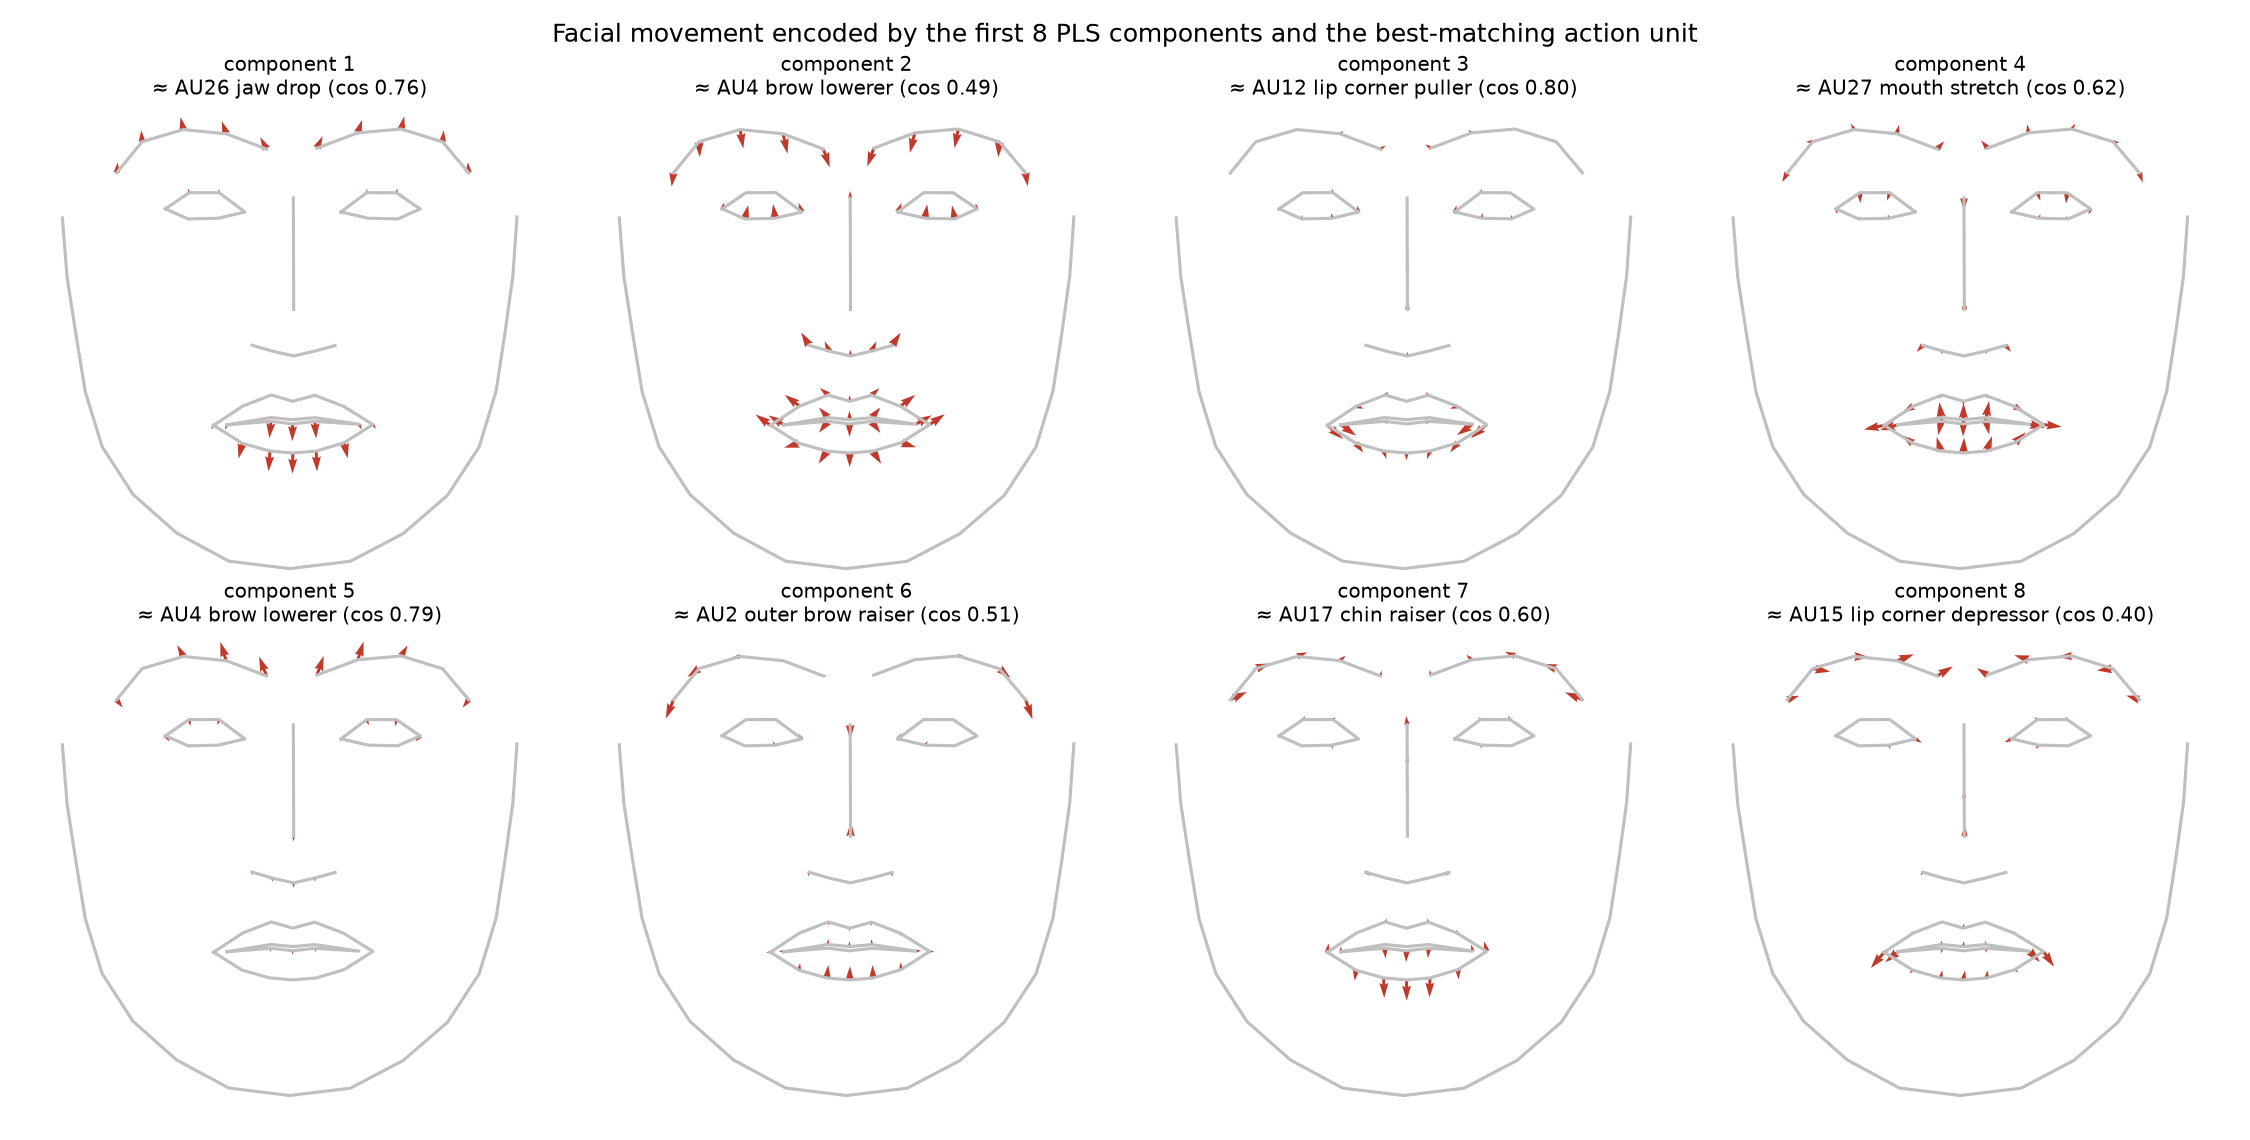
\includegraphics[width=\textwidth]{fig2_components.png}
  \caption{Facial movement encoded by the first eight PLS components (arrows), with the
  best-matching action-unit template.}
  \label{fig:components}
\end{figure}

The leading components are recognisable action units (Figure~\ref{fig:components}): component~1
matches AU26 jaw drop (cosine 0.76), component~3 AU12 lip-corner puller (0.80), component~4 AU27
mouth stretch (0.62), component~5 AU4 brow lowerer (0.79) and component~7 AU17 chin raiser (0.60),
against a random-direction 95th percentile of 0.31. Table~\ref{tab:blocks} summarises the
components in blocks.

\begin{table}[h]
  \centering\small
  \caption{PLS components in blocks.}\label{tab:blocks}
  \begin{tabular}{lcccc}
    \toprule
    Components & Match an AU ($>$ null 95\%) & Localised & Replicability & Median SNR \\
    \midrule
    1--10  & 10/10 & 8/10 & 0.90 & 12.6 \\
    11--20 & 8/10  & 4/10 & 0.84 & 2.8 \\
    21--31 & 2/11  & 5/11 & 0.66 & 2.2 \\
    32--45 & 1/14  & 3/14 & 0.57 & 1.8 \\
    46--60 & 0/15  & 5/15 & 0.47 & 0.7 \\
    \bottomrule
  \end{tabular}
\end{table}

\begin{figure}[t]
  \centering
  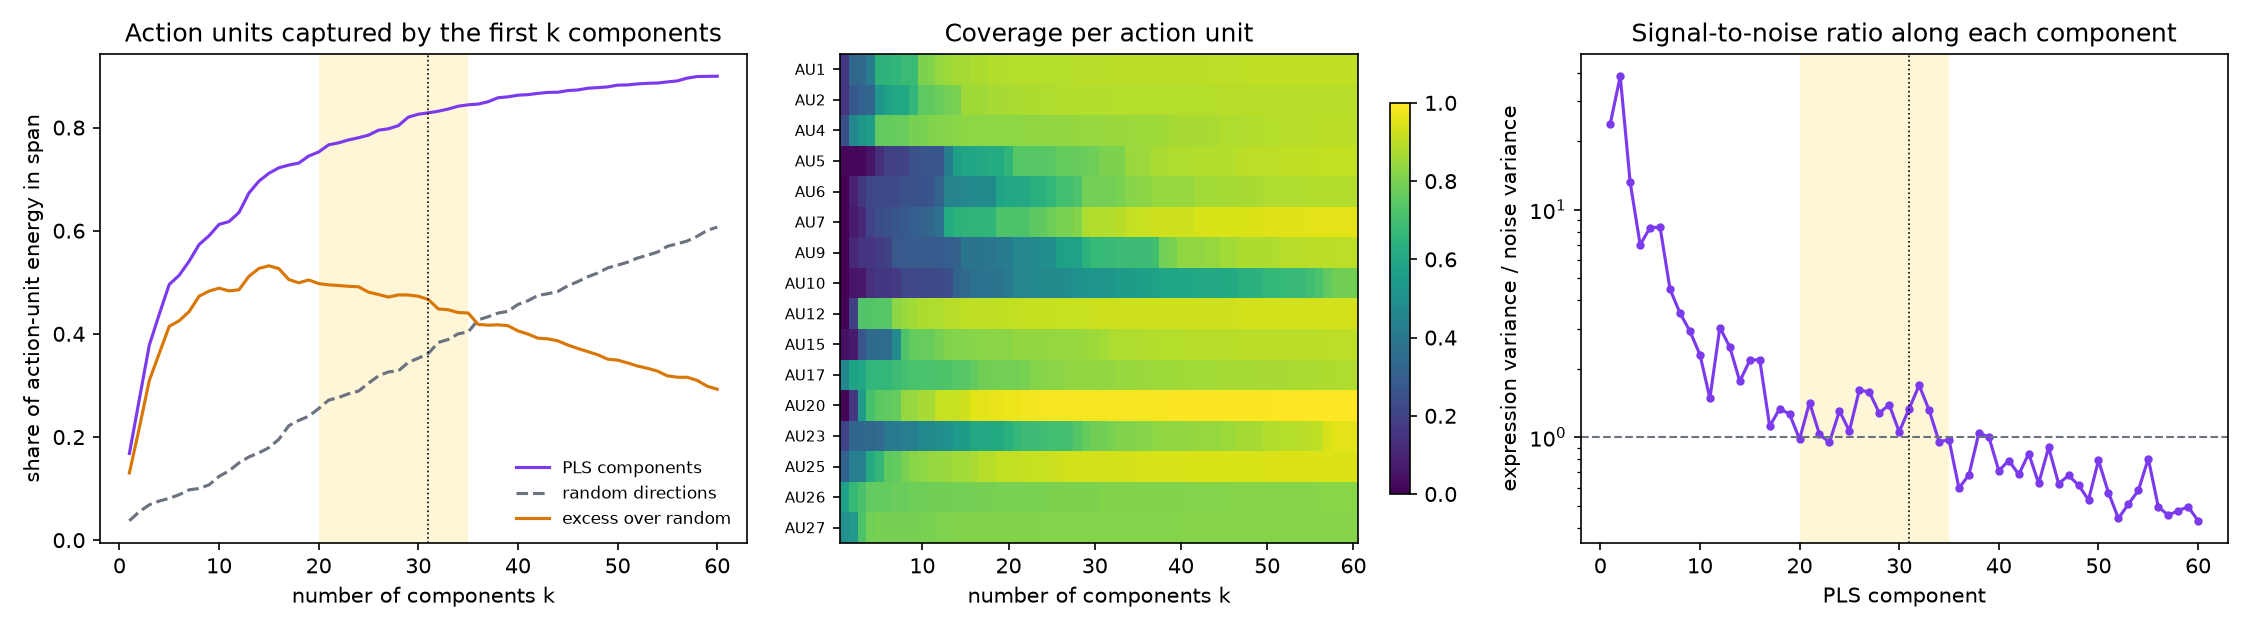
\includegraphics[width=\textwidth]{fig3_coverage_snr.png}
  \caption{Left: share of 16 AU templates captured by the first $k$ components (blue), by $k$
  random directions (grey), and the difference (orange). Middle: coverage per AU. Right: SNR along
  each component, with SNR 1 (dashed) and 2 (dotted). Shaded: components 20--35; dotted vertical
  line: $k = 31$.}
  \label{fig:coverage}
\end{figure}

The span of the first $k$ components captures far more of the AU templates than random directions
do (Table~\ref{tab:coverage}). The excess peaks at 0.53 around $k = 15$ and declines steadily after
about 30; beyond that, further components add no more AU structure than random directions.

\begin{table}[h]
  \centering\small
  \caption{Share of AU-template energy in the span of the first $k$ components.}\label{tab:coverage}
  \begin{tabular}{lccccc}
    \toprule
    $k$ & 10 & 20 & 31 & 40 & 60 \\
    \midrule
    PLS    & 0.61 & 0.75 & 0.83 & 0.86 & 0.90 \\
    Random & 0.12 & 0.26 & 0.36 & 0.46 & 0.61 \\
    Excess & 0.49 & 0.50 & 0.47 & 0.41 & 0.29 \\
    \bottomrule
  \end{tabular}
\end{table}

Coverage per AU (Figure~\ref{fig:coverage}, middle) shows the order in which AUs are learnt:
\begin{itemize}
  \item \textbf{Large mouth and brow movements first.} AU12, AU20, AU25, AU1, AU2 and AU4 reach
  75--88\% within 10 components.
  \item \textbf{Eyelid AUs late.} AU5 upper lid raiser (0.27 at $k = 10$, 0.65 at 20, 0.80 at 31),
  AU6 cheek raiser (0.25, 0.60, 0.79) and AU7 lid tightener (0.31, 0.72, 0.88) are only covered by
  components 20--31. Their landmark displacements are a few pixels, close to the noise.
  \item \textbf{Two AUs remain poorly covered} even at $k = 31$: AU9 nose wrinkler (0.67) and AU10
  upper lip raiser (0.53). Their landmark signature is small and overlaps with neighbouring AUs.
\end{itemize}

\begin{figure}[t]
  \centering
  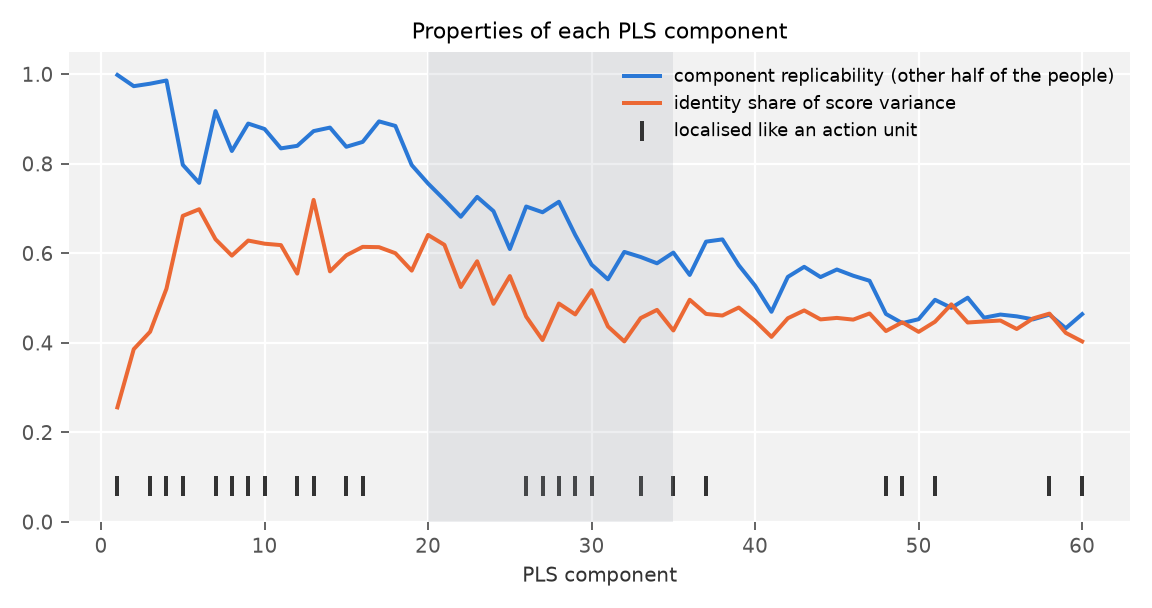
\includegraphics[width=0.62\textwidth]{fig4_component_properties.png}
  \caption{Per-component replicability across disjoint halves of the people, identity share of the
  score variance, and components localised like an AU.}
  \label{fig:properties}
\end{figure}

Components 5--20 have an identity share of 0.55--0.72 (Figure~\ref{fig:properties}): their scores
vary more between people's neutral faces than with expression. These are directions where identity
and expression overlap, such as brow height, and PLS must model them to separate the two.
Replicability drops from about 0.88 to about 0.68 between components 18 and 22. The subspace
spanned by the first $k$ components stays stable (mean squared cosine 0.94 at $k = 20$, 0.91 at 31,
0.85 at 60), so late components are individually unstable even though the space they add is not
arbitrary.

\subsection{Along PLS components, the SNR falls from about 13 to 1--3 after component 20}

PLS orders components by their covariance with the targets, not by SNR, so the SNR along components
is not monotonic (Figure~\ref{fig:coverage}, right). Its trend matches the dimension count:
\begin{itemize}
  \item \textbf{Components 1--19:} SNR 2.1--50 (median 12.6 for 1--10). Expression movement along
  them is many times larger than the noise.
  \item \textbf{Components 20--50:} the SNR fluctuates, mostly between 1 and 5 (median 2.2 for
  21--31, 1.8 for 32--45), with five components (20, 40, 42, 44, 48) below 1. In all, 30 components
  have SNR $\ge 2$, the same number as the noise-whitened directions of Table~\ref{tab:dims}.
  \item \textbf{Components after 50:} the SNR is below 1 for all ten; noise dominates.
\end{itemize}
The components that are recognisable action units (1--20) are thus those with high SNR. Components
20--50 encode real but small movements, such as the eyelid AUs, at an SNR of about 1--3; they no
longer match single AUs and replicate less well across people.

\subsection{Noise sets the accuracy-optimal complexity}\label{sec:noise-accuracy}

\begin{figure}[t]
  \centering
  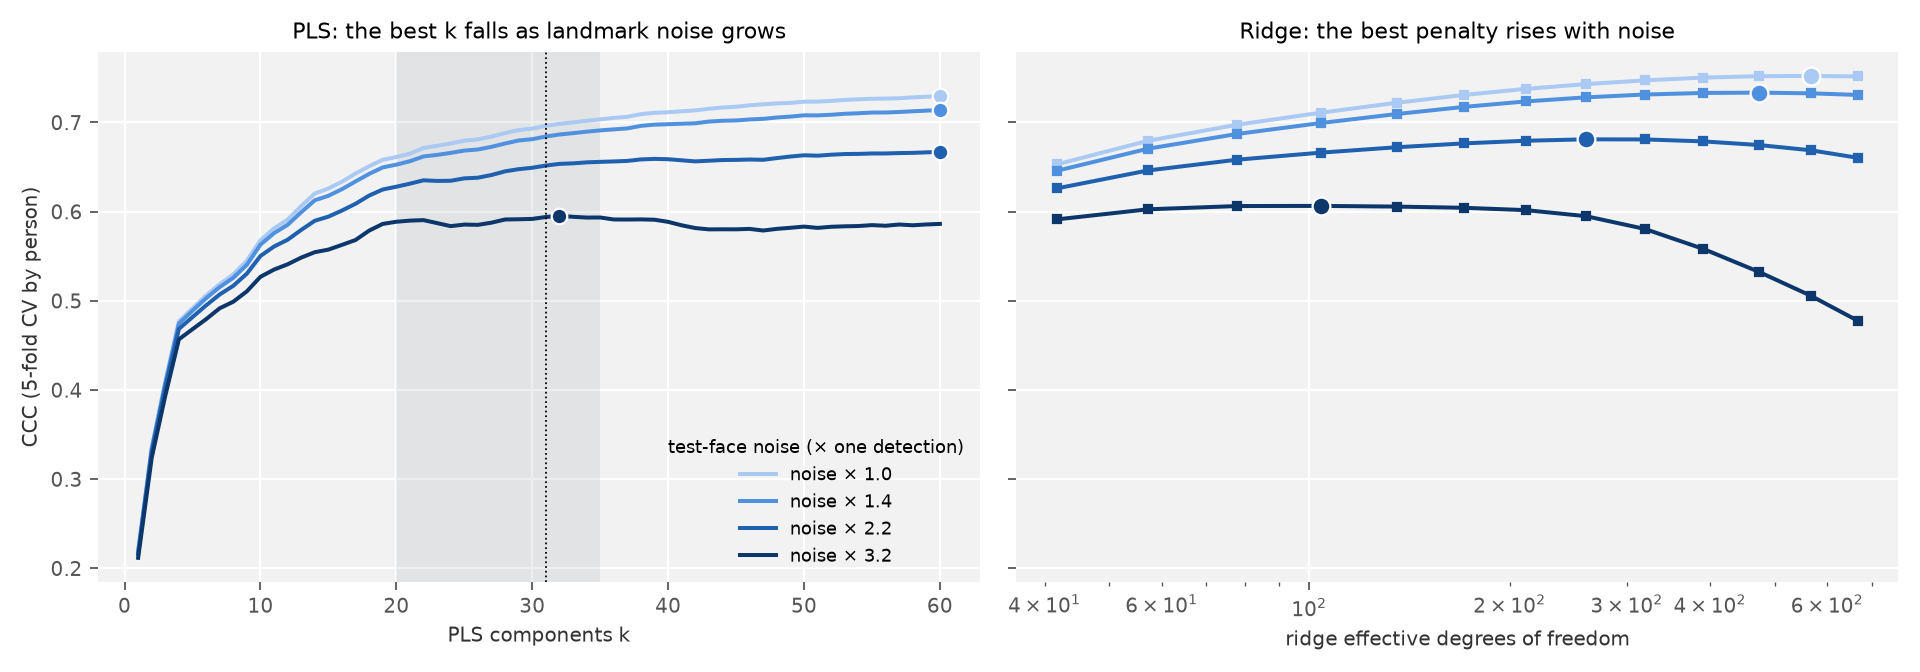
\includegraphics[width=\textwidth]{fig5_noise_accuracy.png}
  \caption{Cross-validated CCC on test faces with extra measured landmark noise (total noise in
  multiples of one detection; dots: maximum). Left: PLS by number of components. Right: ridge by
  effective degrees of freedom.}
  \label{fig:noise-accuracy}
\end{figure}

\begin{table}[h]
  \centering\small
  \caption{Accuracy (CCC) on test faces with more landmark noise.}\label{tab:noise-accuracy}
  \begin{tabular}{lcccc}
    \toprule
    Test-face noise ($\times$ one detection) & 1.0 & 1.4 & 2.2 & 3.2 \\
    Comparable live condition (original detector) & photos & -- & dim & night \\
    \midrule
    Best PLS $k$ (CCC) & 60 (0.730) & 60 (0.714) & 60 (0.667) & \textbf{32} (0.595) \\
    Smallest PLS $k$ within 0.005 of best & 53 & 53 & 50 & 22 \\
    CCC of PLS(31) & 0.696 & 0.684 & 0.652 & 0.594 \\
    Best ridge, effective df (CCC) & 567 (0.752) & 473 (0.733) & 260 (0.681) & \textbf{104} (0.606) \\
    Kernel ridge CCC & 0.757 & 0.743 & 0.703 & 0.639 \\
    \bottomrule
  \end{tabular}
\end{table}

The more noise the test faces carry, the simpler the best linear model
(Figure~\ref{fig:noise-accuracy}, Table~\ref{tab:noise-accuracy}). For ridge, the optimal effective
degrees of freedom fall steadily from 567 to 473, 260 and 104; at 3.2 times the noise, the optimum
is the same ridge model that behaves like PLS(31) in Section~\ref{sec:behaviour}. For PLS, the CCC
curve flattens and then turns over: at 3.2 times the noise the maximum is at 32 components, and
everything from 22 components on is within 0.005 of it. Highly complex models collapse; lightly
penalised ridge (668 df) falls from 0.751 to 0.477.

This is the clearest answer to Q3. Offline evaluation on still photographs measures accuracy at the
photos' noise level, where many weak directions still pay off. A live webcam with the original
detector runs at 1.6--3.2 times that noise (Table~\ref{tab:webcam}). There, accuracy itself selects
a model of about 30 components: the 2021 choice of PLS(31), made by watching the live demo, is what
cross-validation would have chosen had it been run at webcam noise.

The kernel model stays the most accurate at every noise level. Noise explains how complex a linear
model should be, but not the kernel model's live problems, which concern consistency.

\subsection{Accuracy versus live behaviour}\label{sec:behaviour}

\begin{figure}[t]
  \centering
  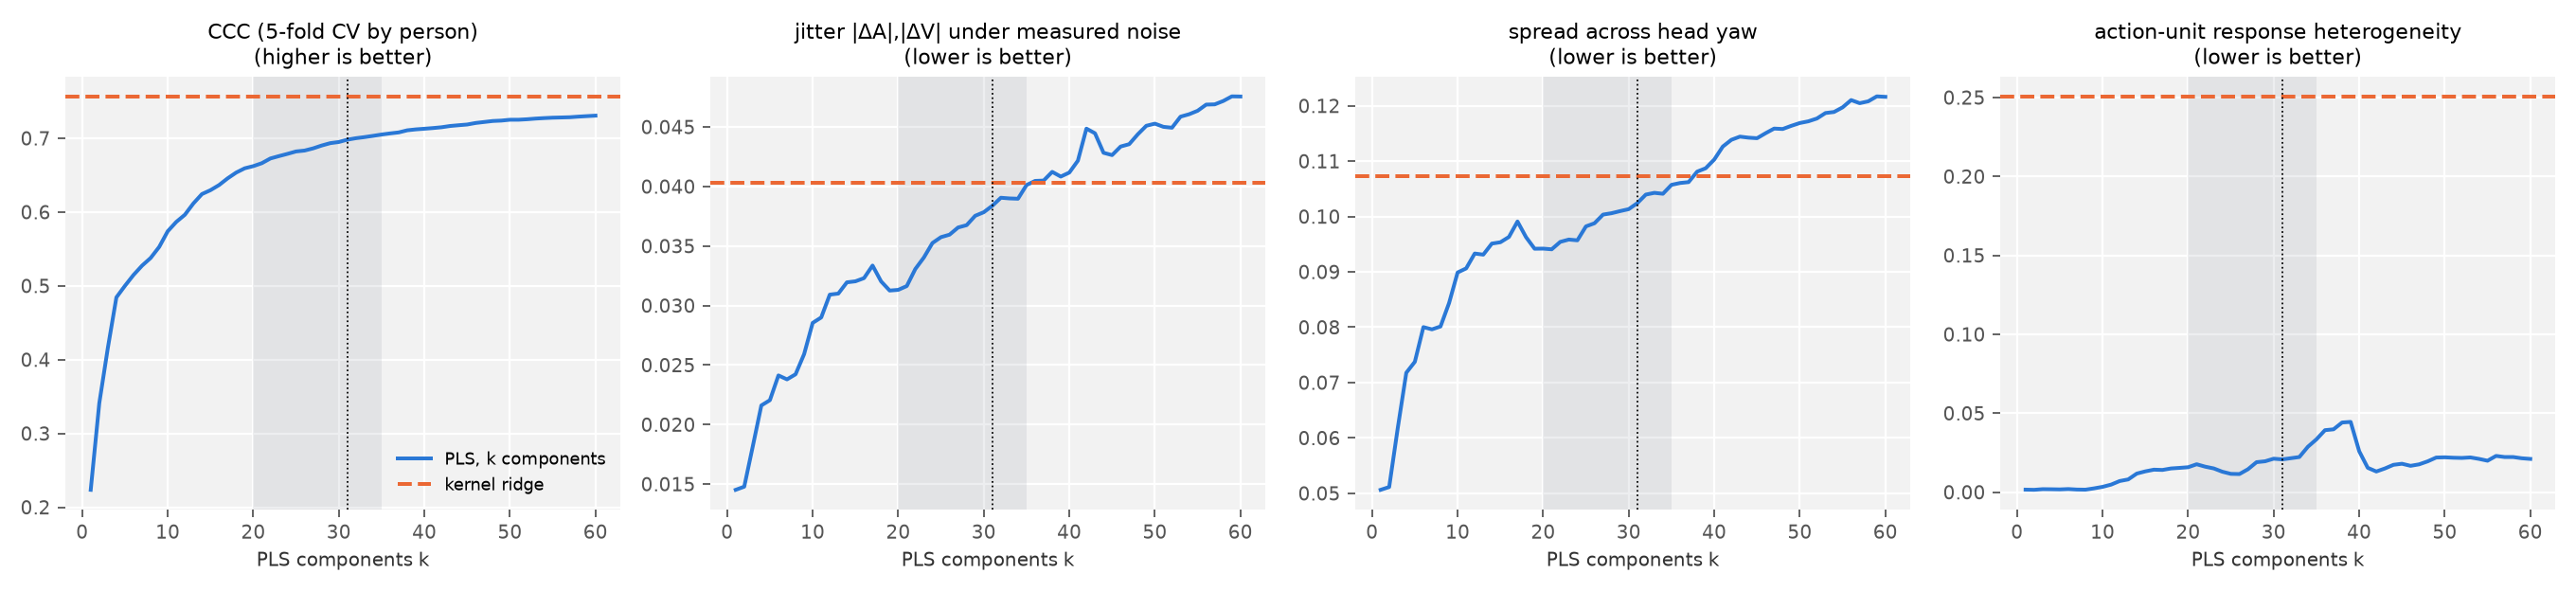
\includegraphics[width=\textwidth]{fig6_tradeoff.png}
  \caption{As the number of PLS components grows (blue), CCC rises steadily, but jitter and pose
  sensitivity rise with it. Kernel ridge (orange, dashed) is the most accurate, but its response to
  action units depends on the face.}
  \label{fig:tradeoff}
\end{figure}

\begin{table}[h]
  \centering\small
  \caption{Accuracy and behaviour. Jitter is at the noise of one detection and scales roughly in
  proportion to the noise.}\label{tab:behaviour}
  \begin{tabular}{lcccccc}
    \toprule
    Model & CCC & $\Delta$CCC & Identity leak. & AU heterog. & Jitter & Pose sens. \\
    \midrule
    PLS(10) & 0.574 & 0.428 & 0.143 & 0.003 & 0.029 & 0.090 \\
    PLS(20) & 0.662 & 0.523 & 0.144 & 0.016 & 0.031 & 0.094 \\
    \textbf{PLS(31)} & 0.698 & 0.555 & 0.140 & 0.021 & 0.038 & 0.102 \\
    PLS(50) & 0.725 & 0.580 & 0.145 & 0.022 & 0.045 & 0.117 \\
    Ridge, $\alpha = 3\cdot10^{-3}$ (104 df) & 0.713 & 0.564 & \textbf{0.133} & 0.023 & 0.038 & \textbf{0.099} \\
    Ridge, $\alpha = 10^{-7}$ (668 df) & 0.751 & 0.617 & 0.189 & 0.053 & 0.057 & 0.146 \\
    Kernel ridge & \textbf{0.757} & 0.615 & 0.176 & \textbf{0.251} & 0.040 & 0.107 \\
    \bottomrule
  \end{tabular}
\end{table}

\paragraph{Accuracy rises with complexity.} For PLS, CCC goes from 0.57 ($k = 10$) to 0.70 (31) and
0.73 (60); lightly penalised ridge and kernel ridge reach 0.75--0.76 (Table~\ref{tab:behaviour}).
This is the offline result that favours complex models.

\paragraph{Linear models: complexity costs jitter and pose stability.} Jitter rises from 0.029
($k = 10$) to 0.038 (31) and 0.048 (60) for PLS, and from 0.029 to 0.057 along the ridge path. Pose
sensitivity rises from 0.090 to 0.102 and 0.122. Both follow from the SNR analysis: components with
an SNR near 1 add almost as much landmark noise as signal to every prediction, and shape changes
that frontalization leaves behind after a head turn project onto them as well.

\paragraph{Kernel ridge: a different failure.} Its jitter (0.040) is close to PLS(31)'s. Its
weakness is consistency across faces: the same synthetic AU changes its output differently on
different faces (heterogeneity 0.25, against 0.02 for linear models), and its predictions for
neutral faces vary more between people (0.176 vs 0.140). A linear model in distance space responds
to a movement almost identically on every face; its small heterogeneity comes from the
non-linearity of the distances. A kernel model's response depends on how close a face is to its
training faces.

\paragraph{The kernel's offline gain is not identity fitting.} Its advantage also holds for
within-person responses ($\Delta$CCC 0.615 vs 0.555 for PLS(31)), so it is not explained by fitting
person-specific offsets. On MorphSet the kernel model is genuinely more accurate; the open question
is what it does on faces and conditions unlike its training data.

\begin{figure}[t]
  \centering
  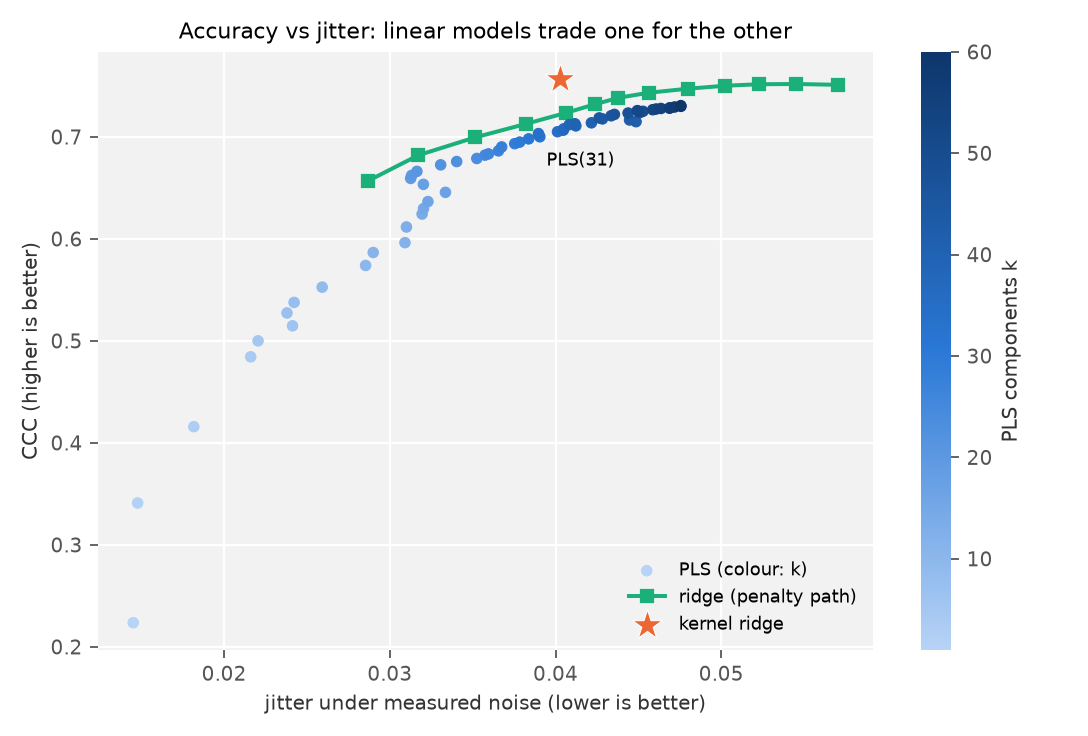
\includegraphics[width=0.62\textwidth]{fig7_pareto.png}
  \caption{Accuracy against jitter. Along the ridge penalty path (green) and the PLS component path
  (coloured by $k$), accuracy is bought with jitter. Kernel ridge (star) lies off this frontier:
  accurate and stable, but not consistent across faces.}
  \label{fig:pareto}
\end{figure}

\paragraph{PLS is not special.} Ridge with $\alpha = 3\cdot10^{-3}$ has the same jitter as PLS(31)
(0.038), higher CCC (0.713 vs 0.698), lower identity leakage (0.133 vs 0.140), lower pose
sensitivity (0.099 vs 0.102) and similar heterogeneity (Figure~\ref{fig:pareto}). Its effective
degrees of freedom (104) exceed 31, but PLS's own degrees of freedom are known to exceed its number
of components \citep{kramer2011degrees}, and PLS and ridge shrink in similar ways
\citep{frank1993statistical}. What matters is the effective complexity of a regularised linear
model, not the PLS algorithm.

% ==========================================================================================
\section{Discussion}

\subsection{The story in one paragraph}

A face seen through 51 landmarks moves along a few dominant directions (mouth opening, smile,
brows) and a longer tail of smaller ones (eyelids, nose, lip details). Dlib measures each landmark
with about 1\,px of error, which fixes how many directions can be measured reliably: about 20
strong ones and 30 with signal at least twice the noise. PLS finds the strong ones first, and they
turn out to be action units. After about 20 components it moves into the tail, where signal and
noise are comparable. Whether these tail components help depends on the noise. On clean
photographs averaged over 80,000 faces, they still add accuracy. On a webcam, whose noise is
1.6--3.2 times larger with the original detector, they add more noise than signal, and the most
accurate model has about 30 components. On top of that, each extra component makes the output shake
more and depend more on head pose, which a user sees but an average error does not show. PLS(31)
sits where the reliable directions end. It was chosen by eye in 2021, and the analysis shows why
the eye was right.

\subsection{Why offline accuracy and live behaviour disagree}

There are three distinct reasons, in decreasing order of importance in our data.
\begin{enumerate}
  \item \textbf{Different noise.} Offline evaluation uses still photographs with one detection's
  noise; live frames carry more. The accuracy-optimal complexity falls as noise rises
  (Section~\ref{sec:noise-accuracy}), so a model tuned on photos is too complex for the webcam.
  \item \textbf{Different loss.} Cross-validated CCC is an average over tens of thousands of faces.
  A user instead sees one face frame by frame, where noise in weak directions appears as jitter;
  their own neutral face, where identity leakage appears as a personal offset; and their own
  movements, where inconsistency appears as trajectories that bend. Temporal variation is far more
  visible than a constant bias of the same size, and calibration removes the bias but not the
  variation. A live loss therefore weights jitter more heavily than MSE does, which favours even
  simpler models.
  \item \textbf{Different faces.} Live users differ from the training faces. Linear models in
  distance space respond to a movement the same way on every face; a kernel model does not.
\end{enumerate}
Temporal smoothing reduces jitter at the cost of lag. A model that jitters less needs less smoothing
and can react faster.

\subsection{The ``coincidence'' with action units}

FACS defines 44 action units, of which about 30 correspond to contractions of specific facial
muscles, 12 in the upper face and 18 in the lower face \citep{tian2001recognizing}. Not all of them
move the 51 landmarks used here; AU11 (nasolabial deepener) and AU14 (dimpler), for example, leave
them almost unchanged. By our estimate roughly 20--25 are landmark-visible, and symmetric and
asymmetric versions of some add further directions. The measured dimensions are of the same order:
about 20 directions with SNR $>$ 4 and AU-aligned PLS components up to about 20; about 30
directions with SNR $>$ 2 and 30 PLS components with SNR $\ge 2$; and a CCC-optimal PLS model of
about 30 components at webcam noise.

We read the coincidence as two descriptions of one quantity: \emph{the number of independent
movement patterns the face can produce that the landmark detector resolves above its noise}.
Anatomy sets the number of independently controllable movements, which FACS counts as action
units; detector noise sets how many of them, and how small, are measurable. A variance-driven latent
method such as PLS discovers them in order of amplitude and runs out of reliable ones at about this
count. Two caveats keep this from being an exact equality. Counting depends on resolution: lower
landmark noise, from a tracker or a denser landmark set, would make more of the tail reliable.
And beyond the first few, PLS components cannot be identified with individual AUs; later components
mix several AUs and identity.

\subsection{Implications}

\begin{enumerate}
  \item \textbf{Select models at the noise level of deployment.} Adding measured detector noise to
  the test faces is cheap and needs no new labels; here it moved the optimal ridge penalty by a
  factor of 5 in effective degrees of freedom.
  \item \textbf{Measure the detector's noise.} Mirrored re-detection gives a full noise covariance
  from any image set; the SNR along latent directions then predicts where extra components stop
  paying off.
  \item \textbf{Add behavioural tests alongside accuracy:} jitter under measured noise, identity
  leakage on neutral faces, consistency of the response to synthetic action units, and pose
  sensitivity, all computable without new labels.
  \item \textbf{Prefer linear models in landmark-distance space when consistency matters.} They
  respond to a facial movement the same way on every face.
  \item \textbf{Reduce noise at the source.} A robust detector and tracker bring live noise close to
  photo level (Table~\ref{tab:webcam}), lengthening the reliable tail and allowing somewhat more
  complex models.
\end{enumerate}

\subsection{Limitations}

\begin{itemize}
  \item \textbf{AU templates are hand-made} geometric approximations from FACS descriptions. A test
  against AU-annotated landmark data such as CK+ \citep{lucey2010ckplus} or DISFA
  \citep{mavadati2013disfa} would make the AU correspondence firmer.
  \item \textbf{The twin noise is a lower bound}: it misses errors both detections share, so the
  SNR values are upper bounds and the reliable dimension may be somewhat smaller.
  \item \textbf{The noise of the real-expression data is unknown}, so the whitened count could not
  be applied to it; under the naive count it agrees with MorphSet.
  \item \textbf{Webcam noise is simulated} by measured photo noise at higher amplitude; real webcam
  errors (motion blur, compression) have a different structure, and the calibration rests on a
  simulated video.
  \item \textbf{Synthetic labels}: MorphSet's labels are morph interpolations of posed prototypes,
  and spontaneous expressions may have a different dimensionality.
  \item \textbf{One detector and one landmark set}: the counts are specific to dlib's 68 points and
  the 51 non-jaw landmarks.
  \item \textbf{Live quality is proxied}, not measured with users; a user study would test the link
  directly.
  \item \textbf{Training noise}: models are trained on photo-level data; noise augmentation might
  change the optimum.
  \item \textbf{Degrees of freedom of PLS} are not computed; the ridge comparison is made at matched
  behaviour, not matched degrees of freedom.
\end{itemize}

% ==========================================================================================
\section{Conclusion}

We set out to explain why a 31-component PLS model, chosen in 2021 because 31 resembled the number
of action units and because it looked best live, outperforms more accurate models in a real-time
demo. The explanation comes from measuring the landmark detector's noise directly: mirrored copies
of each image act as independent re-detections, their difference is pure noise, and the expression
signal follows by subtraction. With signal and noise separated, the picture is consistent.
\begin{itemize}
  \item \textbf{The face has a limited number of measurable movements.} Through 51 dlib landmarks
  with about 1\,px of structured noise, expression has about 20 strong and 30 reliable dimensions,
  and identity as many, of similar size.
  \item \textbf{The strong dimensions are action units.} The first $\sim$20 PLS components recover
  them in order of amplitude; after that, AU structure, replicability and SNR fade together.
  \item \textbf{Noise decides how many dimensions to use.} On clean photographs, accuracy rewards
  the weak tail; at the noise of a webcam with the original detector, the accuracy-optimal linear
  model has about 30 components, or an equivalent ridge penalty.
  \item \textbf{Live use penalises complexity further}: jitter and pose sensitivity grow with every
  weak dimension, and a kernel model, although the most accurate, responds differently to the same
  movement on different faces.
  \item \textbf{PLS itself is not the key}: a ridge regression of matched complexity does as well
  or better.
\end{itemize}
The number of action units turned out to be a good proxy for the number of facial movements a
landmark detector can resolve, and the live demo was a more faithful test of the deployment
condition than offline cross-validation. The lesson applies beyond this system: \emph{choose the
complexity of an interactive model at the noise level where it will be used, measure that noise
directly, and test the behaviour users will see, not only the average error.}

\bibliographystyle{plainnat}
\bibliography{references}

\end{document}
